% Adjust these for the path of the theme and its graphics, relative to this file
%\usepackage{beamerthemeFalmouthGamesAcademy}
\usepackage{../../beamerthemeFalmouthGamesAcademy}
\usepackage{multimedia}
\graphicspath{ {../../} }

% Default language for code listings
\lstset{language=C++,
        morekeywords={each,in,nullptr}
}

% For strikethrough effect
\usepackage[normalem]{ulem}
\usepackage{wasysym}
\usepackage{graphicx} %package to manage images

\usepackage{pdfpages}

% http://www.texample.net/tikz/examples/state-machine/
\usetikzlibrary{arrows,automata}


\newcommand{\modulecode}{COMP702}\newcommand{\moduletitle}{Classical Artificial Intelligence}\newcommand{\sessionnumber}{1}

\begin{document}
\title{\sessionnumber: Module Introduction}
\subtitle{\modulecode: \moduletitle}

\begin{frame}
	
\includegraphics[width=1.0\textwidth]{sign-in}
\end{frame}

\frame{\titlepage} 


\begin{frame}{Today's agenda}
	\begin{itemize}
		\item Prototype Due Date
		\item GAM702 assignment
		\item Iterative Development
		\item Ideation
	\end{itemize}
\end{frame}

\begin{frame}{First Prototype - DIY}
\begin{center}
	\Huge{Due Friday 5pm on Week 3!}
\end{center}
\end{frame}

\part{Iterative Development}
\frame{\partpage}

\begin{frame}{Iterative Game Design Process}
	\begin{figure}
		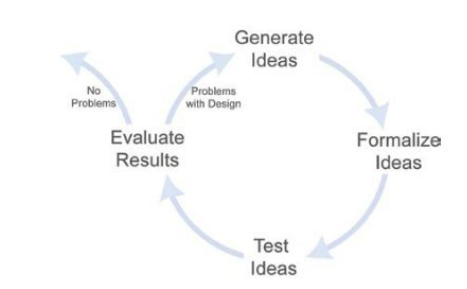
\includegraphics[width=1.0\textwidth,height=0.7\textheight]{iterative_game_design}
		\caption{taken from Game Design Workshop}
		\label{fig:iter1}
	\end{figure}
	\note[item]{Set player experience goals}
\end{frame}

%Set player experience goals
%Brainstorm ideas
%Build a prototype or document system/gameplay etc
%Test ideas (expert or audience)
%Evaluate results
%if idea doesn't work at all, start the process over
%if idea works, modify and test again

\begin{frame}{Design Thinking}
	\begin{figure}
		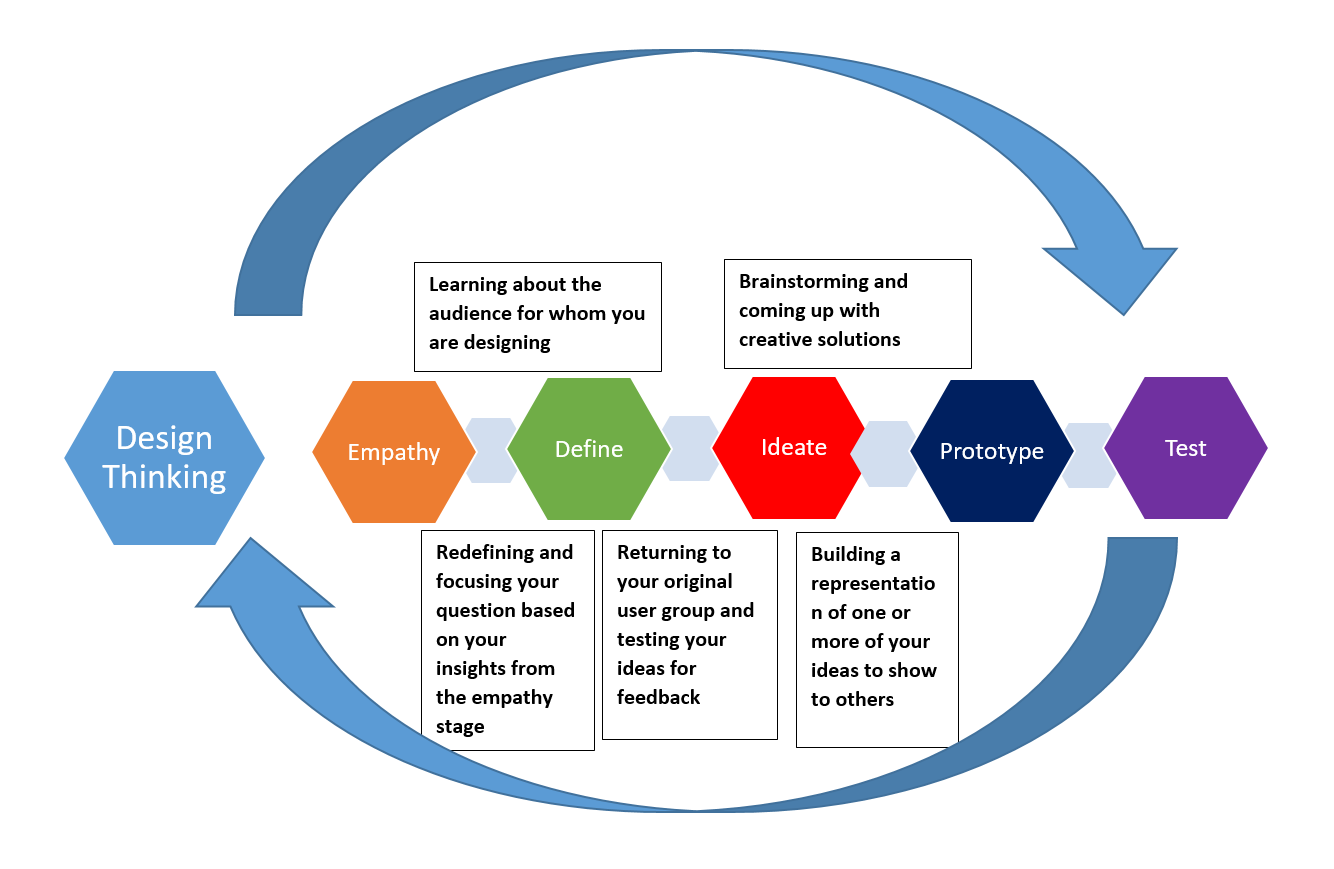
\includegraphics[width=1.0\textwidth, height=0.7\textheight]{design_thinking}
		\label{fig:design_thinking1}
	\end{figure}	
\end{frame}

%important to remember that you can jump around

\begin{frame}{Double Diamond}
	\begin{figure}
		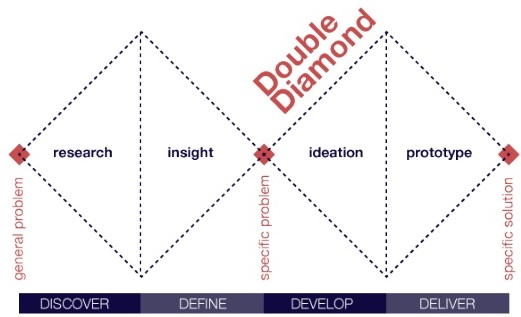
\includegraphics[width=1.0\textwidth, height=0.7\textheight]{double_diamond}
		\label{fig:double_diamond}
	\end{figure}
\end{frame}

%Created by the Design Council
%Discover. The first diamond helps people understand, rather than simply assume, what the problem is. It involves speaking to and spending time with people who are affected by the issues.
%Define. The insight gathered from the discovery phase can help you to define the challenge in a different way.
%Develop. The second diamond encourages people to give different answers to the clearly defined problem, seeking inspiration from elsewhere and co-designing with a range of different people. 
%Deliver. Delivery involves testing out different solutions at small-scale, rejecting those that will not work and improving the ones that will.

\begin{frame}{Summary}
\begin{itemize}
	\item Notice the key similarities in these models
	\item Iteration, testing and revising are key
	\item For the rest of this lecture we are going to focus on the ideation stage
\end{itemize}
\end{frame}
\part{Ideation}
\frame{\partpage}

\begin{frame}{Intro}
	\begin{itemize}
		\item Seen as one of the most important stages
		\item Used to generate challenges
		\item Allows you to explore the possibility space
		\item Challenge assumptions about an area
	\end{itemize}
\end{frame}

\begin{frame}{Brainstorming}
	\begin{columns}
		\begin{column}{0.48\textwidth}
			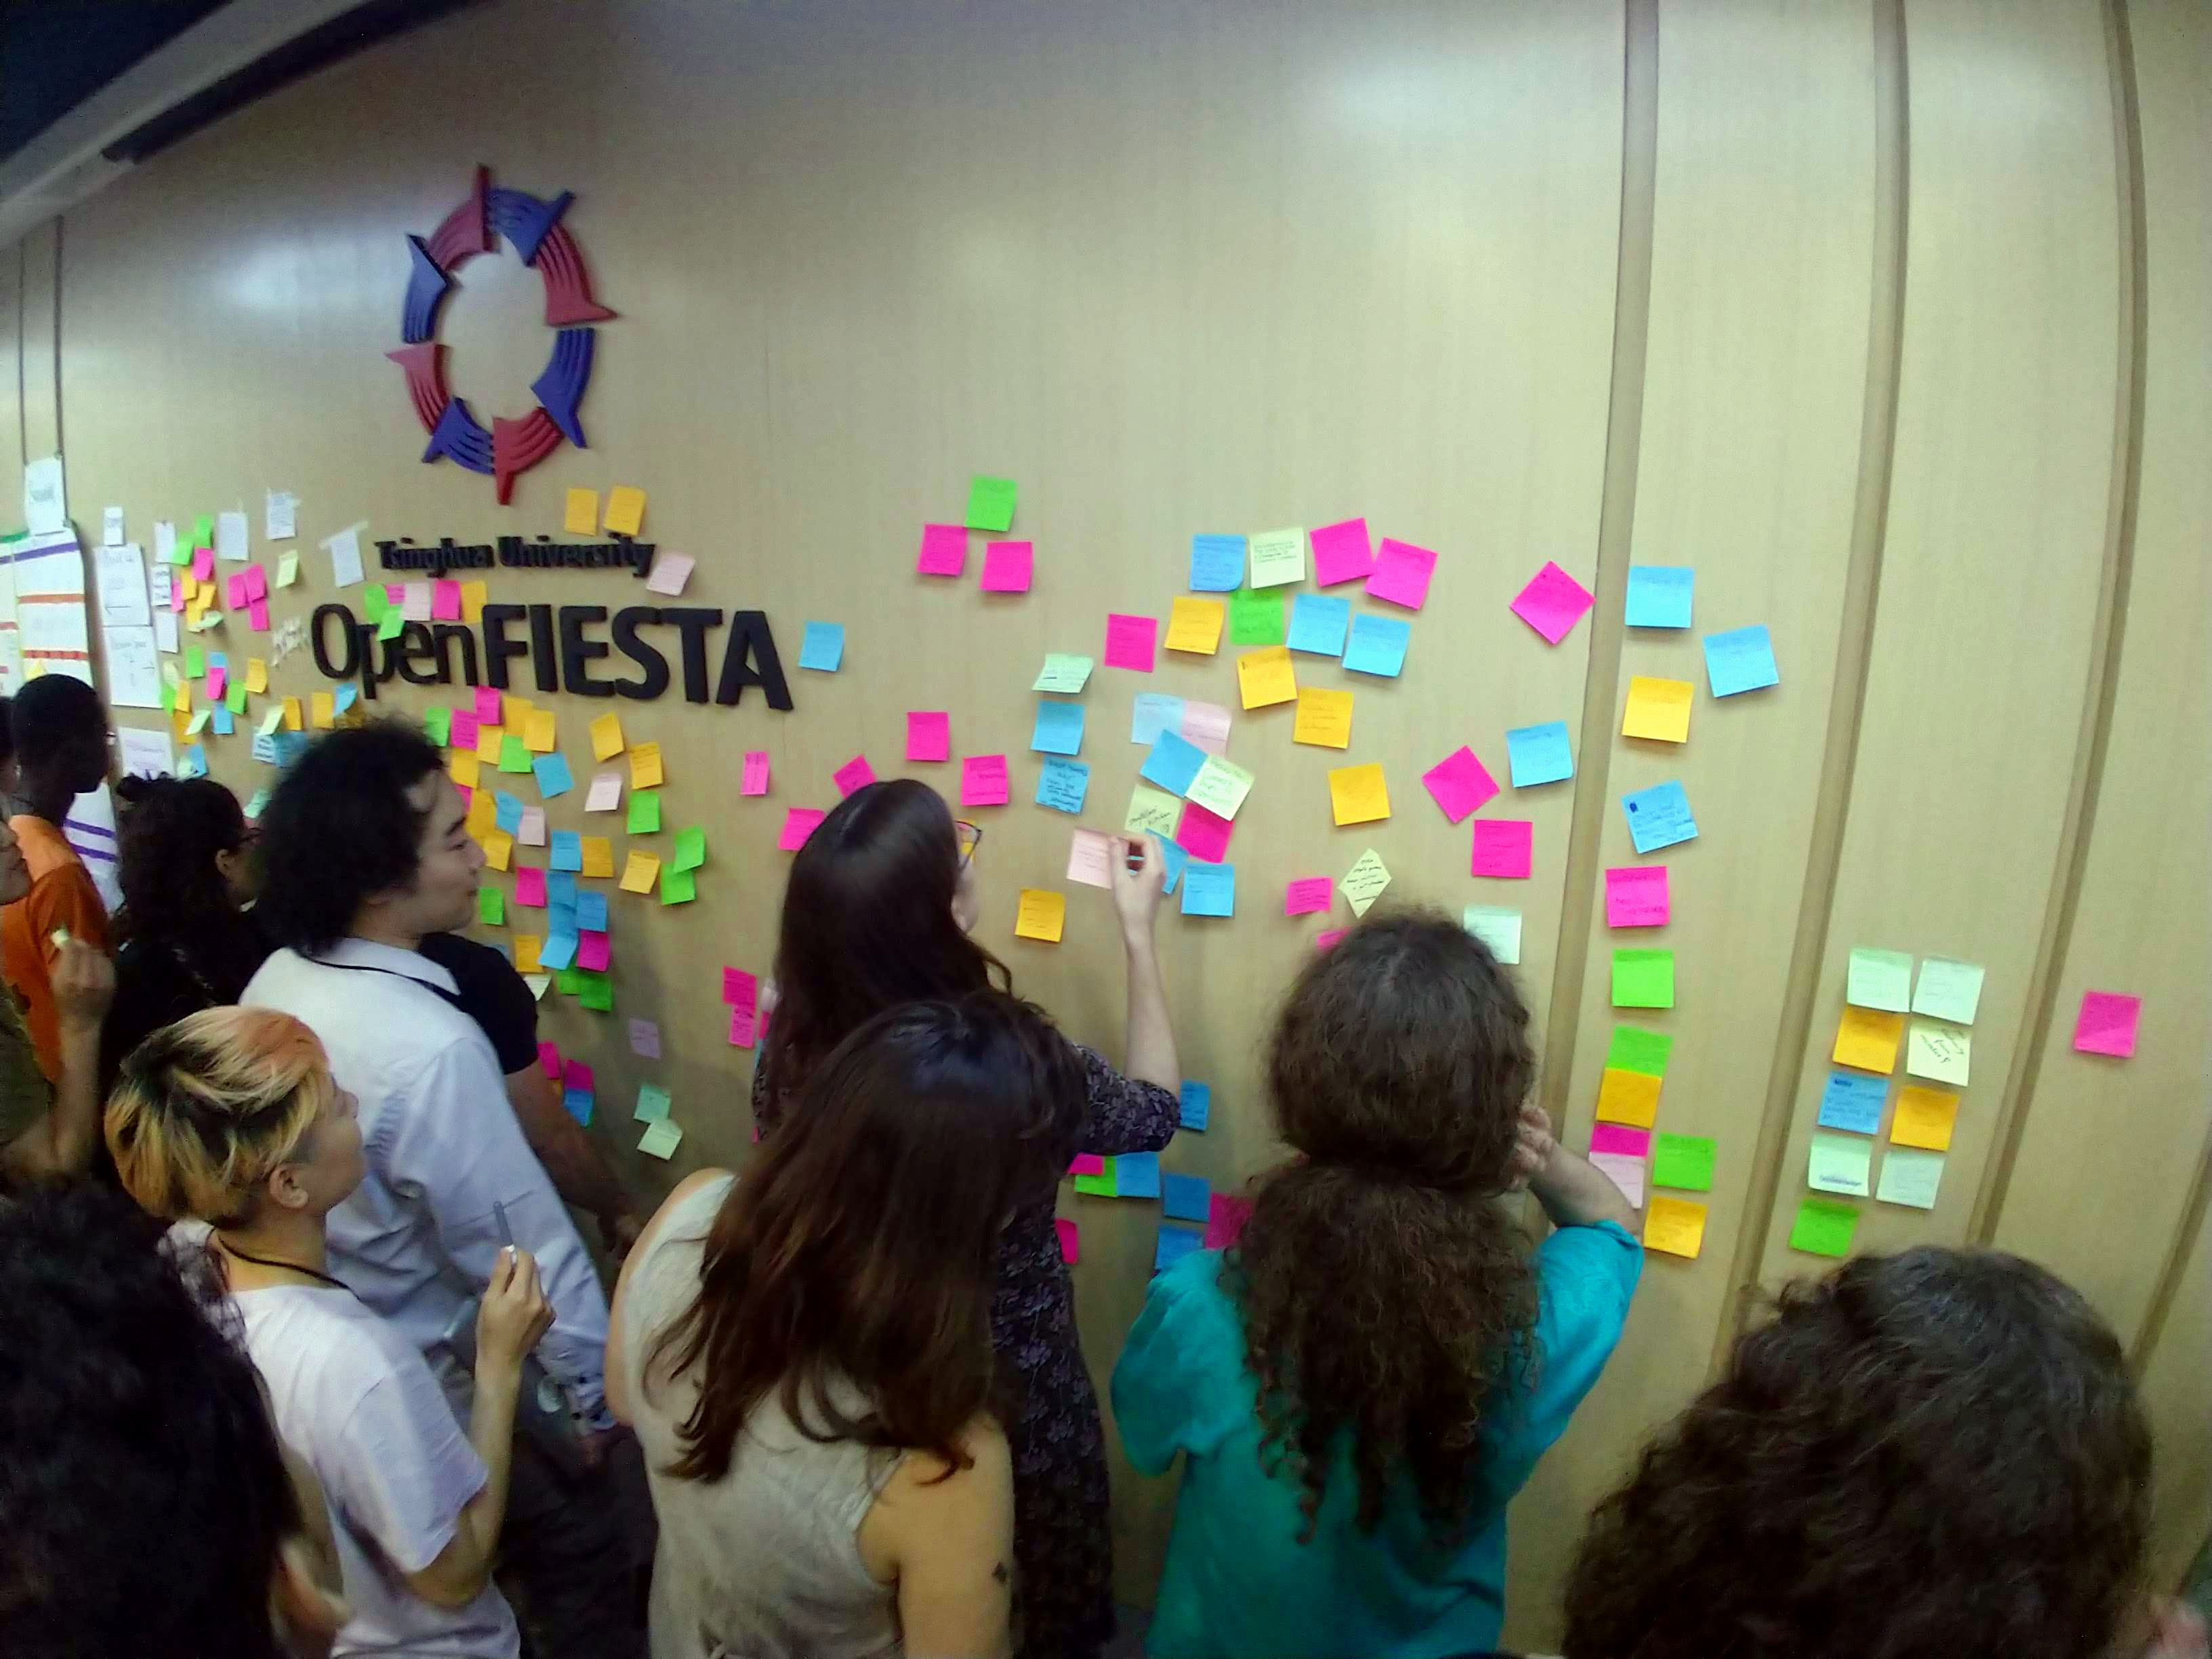
\includegraphics[width=0.9\textwidth, height=0.7\textheight]{brain_storming}
		\end{column}
		\begin{column}{0.48\textwidth}
			\begin{itemize}
				\item First described by Alex Osborn(1953)
			\end{itemize}
			\begin{enumerate}
				\item Idea Quantity
				\item Criticism of the ideas withheld
				\item Wilder the idea, the better
				\item Combine and Improvement
			\end{enumerate}
		\end{column}
	\end{columns}
\end{frame}

\begin{frame}{List Creation}
	\begin{columns}
		\begin{column}{0.48\textwidth}
			\begin{itemize}
				\item Write everything you can about a topic
				\item Free association allows you to explore the area
				\item While organisation of the list allows you to explore relationships 
			\end{itemize}
		\end{column}
		\begin{column}{0.48\textwidth}
			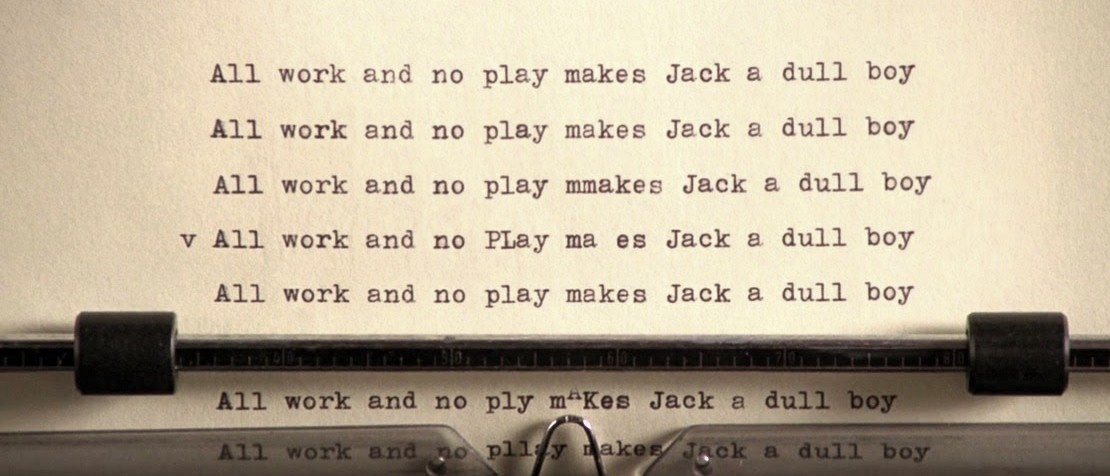
\includegraphics[width=0.9\textwidth, height=0.7\textheight]{list_creation}
		\end{column}
	\end{columns}
\end{frame}

\begin{frame}{Idea/Creativity Cards}
	\begin{columns}
		\begin{column}{0.48\textwidth}
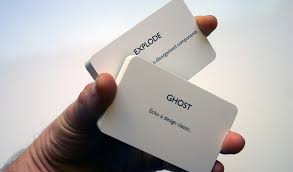
\includegraphics[width=0.9\textwidth, height=0.7\textheight]{creativity_cards}	
		\end{column}
		\begin{column}{0.48\textwidth}
			\begin{itemize}
				\item Start with a blank deck of index cards
				\item Write words on each one
				\item Shuffle the deck, draw two and pair them
				\item Rinse repeat
				\item Or use Creativity Cards
			\end{itemize}
		\end{column}
	\end{columns}
\end{frame}

\begin{frame}{Mind Maps}
	\begin{columns}
		\begin{column}{0.48\textwidth}
			\begin{itemize}
				\item Part of a family of techniques known as \textbf{Concept Mapping}
				\item Demonstrates how people can visualise relationships between topics
				\item Useful for generating a game grammar
			\end{itemize}
		\end{column}
		\begin{column}{0.48\textwidth}
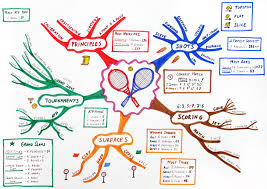
\includegraphics[width=0.9\textwidth, height=0.7\textheight]{mind_map}
		\end{column}
	\end{columns}
\end{frame}

\begin{frame}{Stream of Conscious}
	\begin{columns}
		\begin{column}{0.48\textwidth}
			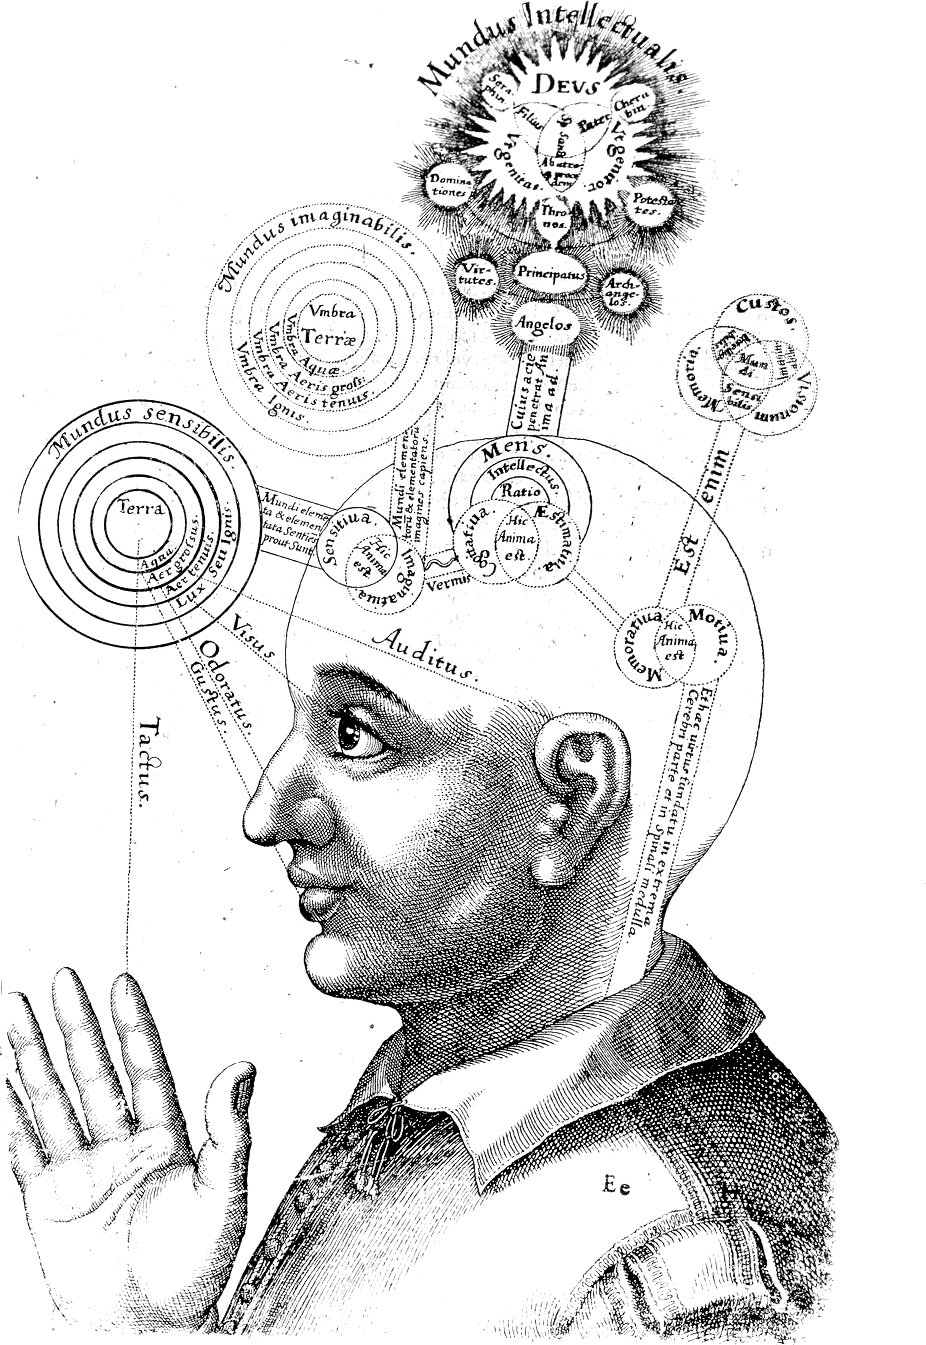
\includegraphics[width=0.9\textwidth, height=0.7\textheight]{stream_of_conscious}
		\end{column}
		\begin{column}{0.48\textwidth}
			\begin{itemize}
				\item Sit down at a computer (or with pen \& paper)
				\item Write everything that comes in mind for 10 mins
				\item Shout out is a variation, which you speak into a voice recorder for 10 mins
			\end{itemize}
		\end{column}
	\end{columns}
\end{frame}

\begin{frame}{Cut it Up}
	\begin{columns}
		\begin{column}{0.48\textwidth}
			\begin{itemize}
				\item Used by the Dadaist art movement e.g. How to Make a Dadaist Poem by Tristan Tzara
				\item Take a magazine or newspaper, cut out word and images
				\item Start playing with pieces and arranging to form ideas
				\item Can lead to surreal juxtapositions 
			\end{itemize}
		\end{column}
		\begin{column}{0.48\textwidth}
			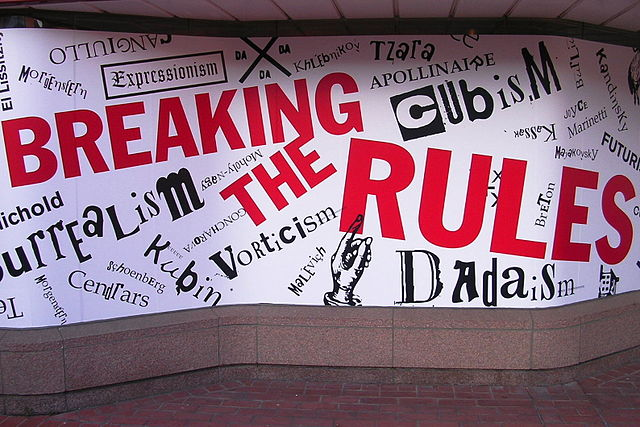
\includegraphics[width=0.9\textwidth, height=0.7\textheight]{cut_up}
		\end{column}
	\end{columns}
\end{frame}

\begin{frame}{Research}
	\begin{columns}
		\begin{column}{0.48\textwidth}
			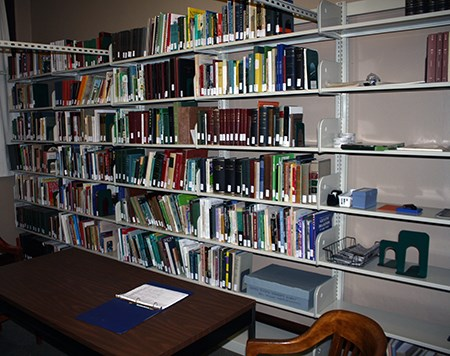
\includegraphics[width=0.9\textwidth, height=0.7\textheight]{research}
		\end{column}
		\begin{column}{0.48\textwidth}
			\begin{itemize}
				\item  Useful for serious games and games that are grounded in a world
				\item Research a topic that interests you. Immerse yourself in a topic
				\item Even if your game isn’t ground in the real world it might have real world analogues
				
			\end{itemize}
		\end{column}
	\end{columns}
\end{frame}

\begin{frame}{Challenge}
\begin{itemize}
	\item For the next Prototype
	\begin{itemize}
		\item Research some of these ideation techniques
		\item Select a couple and use them to generate ideas
		\item Reflect on what games have been created
	\end{itemize}
\end{itemize}
\end{frame}

\begin{frame}{References}
\begin{itemize}
	\item Mongeau, P.A. and Morr, M.C., 1999. Reconsidering brainstorming. Group Facilitation: A Research and Applications Journal, 1(1), pp.14-21.
	\item Lucero, A. and Arrasvuori, J., 2010, September. PLEX Cards: a source of inspiration when designing for playfulness. In Proceedings of the 3rd International Conference on Fun and Games (pp. 28-37). ACM.
	\item Eppler, M.J., 2006. A comparison between concept maps, mind maps, conceptual diagrams, and visual metaphors as complementary tools for knowledge construction and sharing. Information visualization, 5(3), pp.202-210.
	\item Vannucci, M. and Agnoli, S., 2019. Thought Dynamics: Which Role for Mind Wandering in Creativity?. In Dynamic Perspectives on Creativity (pp. 245-260). Springer, Cham.
	\item Weidner, C., 2019. The Glorious Plagiarism, Trash Aesthetics, and Ecological Entropy of Cryptic Cut-Ups from Minutes to Go. Humanities, 8(2), p.116.
\end{itemize}
\end{frame}

\end{document}
